\documentclass[11pt,a4paper]{article}

\usepackage[utf8]{inputenc}
\usepackage[T1]{fontenc}
\usepackage{lmodern}
\usepackage{amsmath,amssymb,mathtools,bm}
\usepackage{graphicx}
\usepackage{float}
\usepackage{subcaption}
\usepackage{geometry}
\usepackage{microtype}
\usepackage{xcolor}
\usepackage{enumitem}
\usepackage{fancyhdr}
\usepackage[hidelinks]{hyperref}

\geometry{top=2.15cm,bottom=2.15cm,left=2.3cm,right=2.3cm}
\setlength{\parindent}{0pt}
\setlength{\parskip}{0.62em}
\setlist[enumerate]{topsep=0.3em,itemsep=0.25em}
\allowdisplaybreaks
\graphicspath{{figures/}}

\definecolor{deepblue}{RGB}{24,62,102}
\hypersetup{
  colorlinks=true,
  linkcolor=deepblue,
  urlcolor=deepblue,
  pdftitle={Teori Gelombang Spin Linear pada Rantai Spiral Satu Dimensi},
  pdfsubject={Derivasi lengkap dari Hamiltonian sampai grafik dispersi dan intensitas}
}

\pagestyle{fancy}
\setlength{\headheight}{14pt}
\fancyhf{}
\fancyhead[L]{Teori Gelombang Spin Linear}
\fancyhead[R]{Rantai Spiral 1D}
\fancyfoot[C]{\thepage}
\renewcommand{\headrulewidth}{0.4pt}

\newcommand{\ii}{\mathrm{i}}
\newcommand{\ee}{\mathrm{e}}
\newcommand{\vq}{\bm q}
\newcommand{\vQ}{\bm Q}
\newcommand{\vS}{\bm S}
\newcommand{\vh}{\bm h}
\newcommand{\vn}{\widehat{\bm n}}
\newcommand{\vD}{\bm D}
\newcommand{\mJ}{\mathsf J}
\newcommand{\mM}{\mathsf M}
\newcommand{\mH}{\mathcal H}
\newcommand{\identity}{\mathsf I}

\title{\textbf{Teori Gelombang Spin Linear pada Rantai Spiral Satu Dimensi}\\[0.35em]
\large Penurunan lengkap dari Hamiltonian sampai dispersi dan peta intensitas $S(\vq,\omega)$}
\author{Catatan terpadu teori semiklasik, teori kuantum, dan linear spin-wave theory}
\date{23 Juli 2026}

\begin{document}
\maketitle

\section{Apa yang akan diturunkan dan konvensi yang dipakai}

Tujuan dokumen ini adalah memperoleh rantai logika berikut tanpa lompatan:
\begin{equation}
\begin{aligned}
H_{\mathrm{spin}}
&\longrightarrow
\text{keadaan dasar klasik}
\longrightarrow
\text{sumbu spin lokal}
\longrightarrow
\text{Holstein--Primakoff}\\
&\longrightarrow
\mH_{\mathrm{BdG}}(q)
\longrightarrow
\varepsilon_n(q)
\longrightarrow
S^{\alpha\beta}(q,\omega)
\longrightarrow
I(q,\omega).
\end{aligned}
\label{eq:master-chain}
\end{equation}
Setiap panah akan diturunkan. Tidak ada nilai numerik coupling, spin, pitch, jumlah titik momentum, lebar broadening, atau koefisien form factor yang diambil dari program pembuat grafik. Gambar yang diberikan dipakai sebagai data visual; hubungannya dengan teori dijelaskan melalui persamaan simbolik.

\subsection{Spin dibuat tak berdimensi, tetapi \texorpdfstring{$\hbar$}{hbar} tetap ditulis}

Operator spin memenuhi
\begin{equation}
[S_i^\alpha,S_j^\beta]
=\ii\,\delta_{ij}\epsilon_{\alpha\beta\gamma}S_i^\gamma.
\label{eq:spin-commutator}
\end{equation}
Dengan konvensi ini, eigenvalue $S_i^z$ adalah $m_i=-S_i,-S_i+1,\ldots,S_i$ dan tidak membawa satuan $\hbar$. Faktor $\hbar$ tetap muncul pada persamaan gerak dan hubungan energi--frekuensi,
\begin{equation}
\varepsilon_n(q)=\hbar\omega_n(q).
\end{equation}

\subsection{Aturan menghitung bond dan asal faktor \texorpdfstring{$1/2$}{1/2}}

Untuk rantai periodik nearest-neighbor, kita gunakan
\begin{equation}
H_J=-J\sum_{i=1}^{N}\vS_i\cdot\vS_{i+1},
\qquad \vS_{N+1}\equiv\vS_1,
\qquad J>0.
\label{eq:fm-hamiltonian}
\end{equation}
Sumasi ini memiliki tepat $N$ bond: $(1,2),(2,3),\ldots,(N,1)$. Setiap bond muncul satu kali.

Jika interaksi ditulis sebagai jumlah terarah atas semua pasangan,
\begin{equation}
H_J=\frac12\sum_{i,j}\vS_i^{T}\mJ_{ij}\vS_j,
\label{eq:directed-sum}
\end{equation}
prefaktor $1/2$ diperlukan karena pasangan $i\to j$ dan $j\to i$ sama-sama muncul. Dengan $\mJ_{ji}=\mJ_{ij}^{T}$,
\begin{equation}
\frac12\left(\vS_i^T\mJ_{ij}\vS_j+\vS_j^T\mJ_{ji}\vS_i\right)
=\vS_i^T\mJ_{ij}\vS_j.
\end{equation}
Inilah alasan faktor $1/2$, bukan angka yang ditambahkan secara bebas.

Apabila Persamaan~\eqref{eq:fm-hamiltonian} sengaja ditulis dua kali,
\begin{equation}
-J\sum_i\left(\vS_i\cdot\vS_{i+1}+\vS_{i+1}\cdot\vS_i\right)
=-2J\sum_i\vS_i\cdot\vS_{i+1},
\end{equation}
seluruh energi eksitasi menjadi dua kali hasil konvensi bond-sekali. Perbedaan faktor dua antara beberapa catatan berasal tepat dari pilihan ini.

\section{Penurunan semiklasik untuk feromagnet satu dimensi}

\subsection{Keadaan dasar}

Pada pendekatan semiklasik, $\vS_i$ diperlakukan sebagai vektor dengan panjang tetap $S$. Untuk satu bond,
\begin{equation}
-J\vS_i\cdot\vS_{i+1}
=-JS^2\cos\theta_{i,i+1}.
\end{equation}
Karena $J>0$, energi minimum dicapai ketika $\cos\theta_{i,i+1}=1$, yaitu $\theta_{i,i+1}=0$. Semua spin sejajar. Dengan $N$ bond, energi dasar klasik adalah
\begin{equation}
E_{\mathrm{cl}}=-NJS^2.
\label{eq:fm-classical-energy}
\end{equation}
Faktor $N$ berasal dari jumlah bond, sedangkan $S^2$ berasal dari dot product dua vektor berpanjang $S$.

\subsection{Persamaan gerak dari Hamiltonian}

Persamaan gerak semiklasik yang konsisten dengan persamaan Heisenberg adalah
\begin{equation}
\hbar\frac{d\vS_i}{dt}
=-\vS_i\times\frac{\partial H}{\partial\vS_i}.
\label{eq:classical-eom-general}
\end{equation}
Untuk Persamaan~\eqref{eq:fm-hamiltonian}, spin $\vS_i$ muncul pada bond $(i-1,i)$ dan $(i,i+1)$. Karena
\begin{equation}
\frac{\partial}{\partial\vS_i}\left(-J\vS_{i-1}\cdot\vS_i\right)=-J\vS_{i-1},
\qquad
\frac{\partial}{\partial\vS_i}\left(-J\vS_i\cdot\vS_{i+1}\right)=-J\vS_{i+1},
\end{equation}
maka
\begin{equation}
\frac{\partial H}{\partial\vS_i}
=-J(\vS_{i-1}+\vS_{i+1}).
\end{equation}
Substitusi ke Persamaan~\eqref{eq:classical-eom-general} memberi
\begin{equation}
\boxed{
\hbar\frac{d\vS_i}{dt}
=J\vS_i\times(\vS_{i-1}+\vS_{i+1}).}
\label{eq:fm-vector-eom}
\end{equation}

\subsection{Linearisasi di sekitar arah \texorpdfstring{$+z$}{+z}}

Ambil keadaan dasar sepanjang $+z$ dan tulis simpangan kecil
\begin{equation}
\vS_i(t)=
\begin{pmatrix}
x_i(t)\\y_i(t)\\S+\delta z_i(t)
\end{pmatrix},
\qquad |x_i|,|y_i|\ll S.
\end{equation}
Syarat panjang spin tetap adalah
\begin{equation}
S^2=x_i^2+y_i^2+(S+\delta z_i)^2
=S^2+2S\delta z_i+x_i^2+y_i^2+\delta z_i^2.
\end{equation}
Sampai orde linear, $x_i^2$, $y_i^2$, dan $\delta z_i^2$ dibuang karena semuanya orde dua. Tersisa $2S\delta z_i=0$, sehingga
\begin{equation}
\delta z_i=0\quad\text{pada orde linear}.
\end{equation}

Komponen $x$ dari cross product adalah
\begin{align}
\left[\vS_i\times(\vS_{i-1}+\vS_{i+1})\right]_x
&=S_i^y(S_{i-1}^z+S_{i+1}^z)
-S_i^z(S_{i-1}^y+S_{i+1}^y)\\
&=y_i(2S)-S(y_{i-1}+y_{i+1})\\
&=S(2y_i-y_{i-1}-y_{i+1}).
\end{align}
Dengan cara yang sama,
\begin{equation}
\left[\vS_i\times(\vS_{i-1}+\vS_{i+1})\right]_y
=-S(2x_i-x_{i-1}-x_{i+1}).
\end{equation}
Komponen $z$ berisi produk $x_iy_j-y_ix_j$, sehingga berorde dua dan dibuang. Persamaan linear lengkap adalah
\begin{align}
\hbar\dot x_i&=JS(2y_i-y_{i-1}-y_{i+1}),\label{eq:fm-x-eom}\\
\hbar\dot y_i&=-JS(2x_i-x_{i-1}-x_{i+1}),\label{eq:fm-y-eom}\\
\hbar\dot z_i&=0.
\end{align}

\subsection{Menggabungkan dua persamaan dan memperoleh dispersi}

Definisikan amplitudo kompleks
\begin{equation}
\psi_i=x_i+\ii y_i.
\end{equation}
Kalikan Persamaan~\eqref{eq:fm-y-eom} dengan $\ii$, lalu jumlahkan dengan Persamaan~\eqref{eq:fm-x-eom}. Karena $y-\ii x=-\ii(x+\ii y)=-\ii\psi$, diperoleh
\begin{equation}
\ii\hbar\dot\psi_i
=JS(2\psi_i-\psi_{i-1}-\psi_{i+1}).
\label{eq:fm-discrete-schrodinger}
\end{equation}

Gunakan gelombang bidang
\begin{equation}
\psi_i(t)=\psi_0\ee^{\ii(kia-\omega t)},
\end{equation}
dengan $a$ jarak antarsitus. Pergeseran satu situs memberi
\begin{equation}
\psi_{i+1}=\psi_i\ee^{\ii ka},
\qquad
\psi_{i-1}=\psi_i\ee^{-\ii ka},
\end{equation}
sedangkan turunan waktu memberi $\dot\psi_i=-\ii\omega\psi_i$. Substitusi ke Persamaan~\eqref{eq:fm-discrete-schrodinger} menghasilkan
\begin{align}
\hbar\omega\psi_i
&=JS\left(2-\ee^{-\ii ka}-\ee^{\ii ka}\right)\psi_i\\
&=JS[2-2\cos(ka)]\psi_i.
\end{align}
Setelah membagi amplitudo tak nol $\psi_i$,
\begin{equation}
\boxed{\hbar\omega(k)=2JS[1-\cos(ka)].}
\label{eq:fm-dispersion}
\end{equation}
Angka $2$ berasal dari identitas $\ee^{\ii x}+\ee^{-\ii x}=2\cos x$ dan dari dua tetangga rantai 1D. Jika Hamiltonian menghitung setiap bond dua kali, ruas kanan Persamaan~\eqref{eq:fm-dispersion} juga menjadi dua kali lebih besar.

Untuk $|ka|\ll1$,
\begin{equation}
\cos(ka)=1-\frac{(ka)^2}{2}+\mathcal O[(ka)^4].
\end{equation}
Maka
\begin{equation}
\hbar\omega(k)
=2JS\left[\frac{(ka)^2}{2}+\mathcal O((ka)^4)\right]
=JSa^2k^2+\mathcal O(k^4).
\label{eq:fm-longwave}
\end{equation}
Faktor $1/2$ dari deret Taylor tepat membatalkan faktor $2$ pada dispersi.

\subsection{Easy-axis anisotropy dan asal gap}

Tambahkan anisotropi
\begin{equation}
H_K=-K\sum_i(S_i^z)^2,
\qquad K>0.
\end{equation}
Turunannya adalah
\begin{equation}
\frac{\partial H_K}{\partial\vS_i}
=-2KS_i^z\widehat{\bm z}.
\end{equation}
Angka $2$ berasal dari turunan $(S_i^z)^2$. Pada orde linear, $S_i^z\simeq S$, sehingga kontribusinya pada persamaan gerak adalah
\begin{equation}
-\vS_i\times\frac{\partial H_K}{\partial\vS_i}
=2KS\vS_i\times\widehat{\bm z}.
\end{equation}
Setelah langkah yang sama seperti sebelumnya,
\begin{equation}
\ii\hbar\dot\psi_i
=JS(2\psi_i-\psi_{i-1}-\psi_{i+1})+2KS\psi_i,
\end{equation}
dan
\begin{equation}
\boxed{\hbar\omega(k)=2JS[1-\cos(ka)]+2KS.}
\label{eq:fm-anisotropy-dispersion}
\end{equation}
Jadi gap pada $k=0$ adalah $2KS$. Apabila anisotropi sejak awal didefinisikan sebagai $-(K/2)(S_i^z)^2$, turunannya hanya menghasilkan $-KS_i^z$ dan gap-nya menjadi $KS$. Perbedaan ini murni akibat definisi koefisien Hamiltonian.

\section{Benchmark antiferomagnet dua sublattice}

Ambil Hamiltonian
\begin{equation}
H_{\mathrm{AF}}=J\sum_i\vS_i\cdot\vS_{i+1},
\qquad J>0.
\end{equation}
Energi satu bond $JS^2\cos\theta$ minimum pada $\theta=\pi$. Keadaan klasiknya adalah pola N\'eel: sublattice $A$ sepanjang $+z$ dan sublattice $B$ sepanjang $-z$.

Letakkan situs $A_n$ pada $2na$ dan $B_n$ pada $(2n+1)a$. Definisikan
\begin{equation}
\psi_{A,n}=x_{A,n}+\ii y_{A,n},
\qquad
\psi_{B,n}=x_{B,n}+\ii y_{B,n}.
\end{equation}
Linearisasi Persamaan~\eqref{eq:classical-eom-general} menghasilkan
\begin{align}
\ii\hbar\dot\psi_{A,n}
&=JS(2\psi_{A,n}+\psi_{B,n-1}+\psi_{B,n}),\\
\ii\hbar\dot\psi_{B,n}
&=-JS(2\psi_{B,n}+\psi_{A,n}+\psi_{A,n+1}).
\end{align}
Tanda yang berbeda berasal dari $S_A^z=+S$ dan $S_B^z=-S$.

Gunakan
\begin{equation}
\psi_{A,n}=u\ee^{\ii(2nka-\omega t)},
\qquad
\psi_{B,n}=v\ee^{\ii[(2n+1)ka-\omega t]}.
\end{equation}
Jumlah dua tetangga memberi
\begin{equation}
\ee^{-\ii ka}+\ee^{\ii ka}=2\cos(ka).
\end{equation}
Maka sistem eigennya adalah
\begin{equation}
\hbar\omega
\begin{pmatrix}u\\v\end{pmatrix}
=2JS
\begin{pmatrix}
1&\cos(ka)\\
-\cos(ka)&-1
\end{pmatrix}
\begin{pmatrix}u\\v\end{pmatrix}.
\end{equation}
Syarat solusi tak nol adalah determinan matriks dikurangi $\hbar\omega\identity$ sama dengan nol:
\begin{align}
0&=\det
\begin{pmatrix}
2JS-\hbar\omega&2JS\cos(ka)\\
-2JS\cos(ka)&-2JS-\hbar\omega
\end{pmatrix}\\
&=(\hbar\omega)^2-(2JS)^2[1-\cos^2(ka)]\\
&=(\hbar\omega)^2-(2JS)^2\sin^2(ka).
\end{align}
Cabang energi positif adalah
\begin{equation}
\boxed{\hbar\omega(k)=2JS|\sin(ka)|.}
\label{eq:af-dispersion}
\end{equation}
Feromagnet memiliki dispersi kuadratik dekat $k=0$, sedangkan antiferomagnet linear karena $|\sin(ka)|\simeq|ka|$. Contoh ini juga menunjukkan mengapa sistem multisublattice menghasilkan matriks, bukan satu persamaan skalar.

\section{Deskripsi kuantum: operator tangga dan satu magnon}

\subsection{Operator tangga tanpa melewati faktor normalisasi}

Definisikan
\begin{equation}
S_i^+=S_i^x+\ii S_i^y,
\qquad
S_i^-=S_i^x-\ii S_i^y.
\end{equation}
Transformasi balik diperoleh dengan menjumlahkan dan mengurangkan kedua persamaan:
\begin{equation}
S_i^x=\frac{S_i^++S_i^-}{2},
\qquad
S_i^y=\frac{S_i^+-S_i^-}{2\ii}.
\end{equation}
Aksinya pada $|S,m\rangle$ adalah
\begin{align}
S^+|S,m\rangle
&=\sqrt{S(S+1)-m(m+1)}\,|S,m+1\rangle,\\
S^-|S,m\rangle
&=\sqrt{S(S+1)-m(m-1)}\,|S,m-1\rangle.
\end{align}
Untuk keadaan paling atas $m=S$,
\begin{equation}
S^-|S,S\rangle
=\sqrt{S(S+1)-S(S-1)}|S,S-1\rangle
=\sqrt{2S}|S,S-1\rangle.
\label{eq:ladder-sqrt2S}
\end{equation}
Jadi $\sqrt{2S}$ berasal langsung dari aljabar momentum sudut.

Dot product dua spin dapat ditulis
\begin{align}
S_i^xS_j^x+S_i^yS_j^y
&=\frac12(S_i^+S_j^-+S_i^-S_j^+),\\
\vS_i\cdot\vS_j
&=S_i^zS_j^z+\frac12(S_i^+S_j^-+S_i^-S_j^+).
\label{eq:spin-dot-ladder}
\end{align}
Faktor $1/2$ muncul setelah ekspansi eksplisit $S^x$ dan $S^y$, bukan asumsi tambahan.

\subsection{Keadaan dasar dan basis satu spin flip}

Untuk Hamiltonian feromagnet Persamaan~\eqref{eq:fm-hamiltonian}, keadaan terpolarisasi penuh adalah
\begin{equation}
|F\rangle=|S,S\rangle_1\otimes\cdots\otimes|S,S\rangle_N.
\end{equation}
Pada setiap bond, operator transversal memusnahkan keadaan ini dan $S_i^zS_{i+1}^z$ memberi $S^2$. Karena ada $N$ bond,
\begin{equation}
H_J|F\rangle=-NJS^2|F\rangle=E_0|F\rangle.
\end{equation}

Definisikan keadaan satu spin flip yang ternormalisasi
\begin{equation}
|j\rangle=\frac{1}{\sqrt{2S}}S_j^-|F\rangle.
\label{eq:one-flip-state}
\end{equation}
Normalisasinya mengikuti Persamaan~\eqref{eq:ladder-sqrt2S}; tanpa faktor $1/\sqrt{2S}$, norm state menjadi $2S$.

Hanya bond $(j-1,j)$ dan $(j,j+1)$ yang berbeda dari ground state. Untuk bond $(j,j+1)$,
\begin{align}
S_j^zS_{j+1}^z|j\rangle&=(S-1)S|j\rangle,\\
\frac12S_j^+S_{j+1}^-|j\rangle&=S|j+1\rangle,\\
\frac12S_j^-S_{j+1}^+|j\rangle&=0.
\end{align}
Baris kedua mempunyai faktor $S$ karena dua aksi operator masing-masing memberi $\sqrt{2S}$, produknya $2S$, lalu dikalikan $1/2$. Bond kiri memberi hasil serupa dengan $|j-1\rangle$.

Setelah bagian ground-state $E_0$ dipisahkan, hasil lengkapnya adalah
\begin{equation}
(H_J-E_0)|j\rangle
=JS\left(2|j\rangle-|j-1\rangle-|j+1\rangle\right).
\label{eq:one-flip-tight-binding}
\end{equation}
Angka $2$ berasal dari dua bond yang menyentuh situs $j$.

\subsection{Transformasi Fourier state satu magnon}

Definisikan state momentum
\begin{equation}
|q\rangle=\frac1{\sqrt N}\sum_{j=1}^{N}\ee^{\ii qR_j}|j\rangle,
\qquad R_j=ja.
\end{equation}
Faktor $1/\sqrt N$ memastikan $\langle q|q\rangle=1$ untuk grid momentum periodik. Terapkan Persamaan~\eqref{eq:one-flip-tight-binding}:
\begin{align}
(H_J-E_0)|q\rangle
&=\frac{JS}{\sqrt N}\sum_j\ee^{\ii qR_j}
\left(2|j\rangle-|j-1\rangle-|j+1\rangle\right).
\end{align}
Pada suku $|j-1\rangle$, ganti indeks $\ell=j-1$, sehingga $R_j=R_\ell+a$ dan faktor fasenya menjadi $\ee^{\ii qa}\ee^{\ii qR_\ell}$. Pada suku $|j+1\rangle$, ganti $\ell=j+1$, sehingga diperoleh $\ee^{-\ii qa}$. Maka
\begin{align}
(H_J-E_0)|q\rangle
&=JS\left(2-\ee^{\ii qa}-\ee^{-\ii qa}\right)|q\rangle\\
&=2JS[1-\cos(qa)]|q\rangle.
\end{align}
Jadi energi satu magnon adalah
\begin{equation}
\boxed{E(q)-E_0=2JS[1-\cos(qa)].}
\end{equation}
Hasil ini identik dengan dispersi semiklasik Persamaan~\eqref{eq:fm-dispersion}. Kesamaan tersebut adalah pemeriksaan konsistensi pertama sebelum masuk ke keadaan spiral yang lebih umum.

\section{Hamiltonian spin umum dan rotasi ke sumbu lokal}

\subsection{Hamiltonian mikroskopik}

Bentuk yang mencakup exchange isotropik, exchange anisotropik, Dzyaloshinskii--Moriya interaction (DMI), anisotropi satu-ion, dan medan adalah
\begin{equation}
H=
\frac12\sum_{i,j}\vS_i^T\mJ_{ij}\vS_j
-\sum_iK_i(\widehat{\bm m}_i\cdot\vS_i)^2
-\sum_i\vh_i\cdot\vS_i.
\label{eq:general-hamiltonian}
\end{equation}
Indeks $i,j$ pada suku pertama adalah jumlah terarah, sehingga prefaktor $1/2$ mengikuti pembahasan Persamaan~\eqref{eq:directed-sum}. Jika hanya bond unik yang dijumlahkan, prefaktor itu dihilangkan.

Matriks coupling dapat dipecah menjadi
\begin{equation}
\mJ_{ij}=J_{ij}\identity_3+\bm\Gamma_{ij}+\mJ_{ij}^{\mathrm{DM}},
\end{equation}
dengan $J_{ij}\identity_3$ bagian Heisenberg isotropik, $\bm\Gamma_{ij}$ bagian simetrik anisotropik, dan
\begin{equation}
\mJ_{ij}^{\mathrm{DM}}=
\begin{pmatrix}
0&D_{ij}^z&-D_{ij}^y\\
-D_{ij}^z&0&D_{ij}^x\\
D_{ij}^y&-D_{ij}^x&0
\end{pmatrix}.
\end{equation}
Perkalian eksplisit menunjukkan
\begin{align}
\vS_i^T\mJ_{ij}^{\mathrm{DM}}\vS_j
={}&D_{ij}^x(S_i^yS_j^z-S_i^zS_j^y)
+D_{ij}^y(S_i^zS_j^x-S_i^xS_j^z)\notag\\
&+D_{ij}^z(S_i^xS_j^y-S_i^yS_j^x)\\
={}&\vD_{ij}\cdot(\vS_i\times\vS_j).
\end{align}
Hermiticity energi bond menuntut
\begin{equation}
\mJ_{ji}=\mJ_{ij}^{T},
\qquad
\vD_{ji}=-\vD_{ij}.
\end{equation}

\subsection{Arah klasik dan basis ortonormal lokal}

Misalkan arah spin klasik pada sublattice $r$ adalah
\begin{equation}
\vn_r=
\begin{pmatrix}
\sin\theta_r\cos\phi_r\\
\sin\theta_r\sin\phi_r\\
\cos\theta_r
\end{pmatrix}.
\label{eq:classical-direction}
\end{equation}
Kita membangun tiga vektor satuan lokal
\begin{align}
\bm e_{r1}&=
\begin{pmatrix}
\cos\theta_r\cos\phi_r\\
\cos\theta_r\sin\phi_r\\
-\sin\theta_r
\end{pmatrix},\\
\bm e_{r2}&=
\begin{pmatrix}
-\sin\phi_r\\
\cos\phi_r\\
0
\end{pmatrix},\\
\bm e_{r3}&=\vn_r.
\end{align}
Masing-masing mempunyai norm satu. Dot product pasangan berbeda juga nol, misalnya
\begin{equation}
\bm e_{r1}\cdot\bm e_{r3}
=\cos\theta_r\sin\theta_r(\cos^2\phi_r+\sin^2\phi_r)
-\sin\theta_r\cos\theta_r=0.
\end{equation}
Maka matriks yang kolomnya ketiga vektor ini,
\begin{equation}
R_r=(\bm e_{r1}\ \bm e_{r2}\ \bm e_{r3})
=
\begin{pmatrix}
\cos\theta_r\cos\phi_r&-\sin\phi_r&\sin\theta_r\cos\phi_r\\
\cos\theta_r\sin\phi_r&\cos\phi_r&\sin\theta_r\sin\phi_r\\
-\sin\theta_r&0&\cos\theta_r
\end{pmatrix},
\label{eq:rotation-matrix}
\end{equation}
memenuhi
\begin{equation}
R_r^TR_r=\identity_3,
\qquad R_r^{-1}=R_r^T,
\qquad \det R_r=1.
\end{equation}

Operator spin global dan lokal dihubungkan oleh
\begin{equation}
\vS_{\ell r}=R_r\widetilde{\vS}_{\ell r}.
\label{eq:global-local-spin}
\end{equation}
Indeks $\ell$ menyatakan magnetic unit cell dan $r$ sublattice di dalamnya. Pada keadaan klasik,
\begin{equation}
\langle\widetilde{\vS}_{\ell r}\rangle=(0,0,S_r)^T,
\end{equation}
karena kolom ketiga $R_r$ adalah arah klasik $\vn_r$.

Untuk bond dari $(\ell,r)$ ke $(\ell+\Delta,s)$,
\begin{align}
\vS_{\ell r}^T\mJ_{rs}(\Delta)\vS_{\ell+\Delta,s}
&=\widetilde{\vS}_{\ell r}^T
R_r^T\mJ_{rs}(\Delta)R_s
\widetilde{\vS}_{\ell+\Delta,s}.
\end{align}
Definisikan coupling dalam frame lokal
\begin{equation}
\boxed{
\mM_{rs}(\Delta)=R_r^T\mJ_{rs}(\Delta)R_s.}
\label{eq:local-coupling}
\end{equation}
Semua kerumitan orientasi klasik sekarang berada di dalam elemen $M_{rs}^{\mu\nu}$.

\section{Transformasi Holstein--Primakoff dan ekspansi orde demi orde}

\subsection{Transformasi eksak dan pendekatan linear spin wave}

Pada setiap sublattice, perkenalkan boson dengan
\begin{equation}
[a_{\ell r},a_{\ell' s}^\dagger]
=\delta_{\ell\ell'}\delta_{rs}.
\end{equation}
Transformasi Holstein--Primakoff eksak adalah
\begin{align}
\widetilde S_{\ell r}^z&=S_r-a_{\ell r}^\dagger a_{\ell r},\label{eq:hp-z}\\
\widetilde S_{\ell r}^+&=\sqrt{2S_r}
\sqrt{1-\frac{a_{\ell r}^\dagger a_{\ell r}}{2S_r}}\,a_{\ell r},\\
\widetilde S_{\ell r}^-&=\sqrt{2S_r}\,
a_{\ell r}^\dagger
\sqrt{1-\frac{a_{\ell r}^\dagger a_{\ell r}}{2S_r}}.
\end{align}
Ekspansi akar
\begin{equation}
\sqrt{1-x}=1-\frac{x}{2}-\frac{x^2}{8}-\cdots
\end{equation}
menunjukkan bahwa koreksi pertama pada $\widetilde S^+$ mengandung tiga operator boson, misalnya $a^\dagger aa$. Linear spin-wave theory mempertahankan Hamiltonian sampai orde dua dalam $a,a^\dagger$, sehingga pada operator spin cukup digunakan
\begin{align}
\widetilde S_{\ell r}^z&=S_r-a_{\ell r}^\dagger a_{\ell r},\\
\widetilde S_{\ell r}^+&\simeq\sqrt{2S_r}\,a_{\ell r},\\
\widetilde S_{\ell r}^-&\simeq\sqrt{2S_r}\,a_{\ell r}^\dagger.
\end{align}

Dengan $\widetilde S^x=(\widetilde S^++\widetilde S^-)/2$ dan $\widetilde S^y=(\widetilde S^+-\widetilde S^-)/(2\ii)$,
\begin{align}
\widetilde S_{\ell r}^x
&=c_r(a_{\ell r}+a_{\ell r}^\dagger),\\
\widetilde S_{\ell r}^y
&=-\ii c_r(a_{\ell r}-a_{\ell r}^\dagger),\\
\widetilde S_{\ell r}^z
&=S_r-n_{\ell r},
\qquad
c_r\equiv\sqrt{\frac{S_r}{2}},
\qquad
n_{\ell r}=a_{\ell r}^\dagger a_{\ell r}.
\label{eq:hp-cartesian}
\end{align}
Faktor $\sqrt{S_r/2}$ berasal dari $\sqrt{2S_r}/2$.

\subsection{Ekspansi lengkap satu bond}

Untuk mempersingkat notasi, tulis $a_r=a_{\ell r}$, $a_s=a_{\ell+\Delta,s}$, dan $M_{\mu\nu}=M_{rs}^{\mu\nu}(\Delta)$. Satu bond adalah
\begin{equation}
H_{rs}=\sum_{\mu,\nu=x,y,z}M_{\mu\nu}\widetilde S_r^\mu\widetilde S_s^\nu.
\end{equation}
Setelah Persamaan~\eqref{eq:hp-cartesian} dimasukkan, kita kelompokkan menurut jumlah operator boson.

Orde nol berasal hanya dari $S_r^zS_s^z$:
\begin{equation}
H_{rs}^{(0)}=M_{zz}S_rS_s.
\label{eq:bond-order0}
\end{equation}

Orde satu berasal dari satu komponen transversal dan satu komponen $z$ klasik:
\begin{align}
H_{rs}^{(1)}={}&
c_rS_s(M_{xz}-\ii M_{yz})a_r
+c_rS_s(M_{xz}+\ii M_{yz})a_r^\dagger\notag\\
&+S_rc_s(M_{zx}-\ii M_{zy})a_s
+S_rc_s(M_{zx}+\ii M_{zy})a_s^\dagger.
\label{eq:bond-order1}
\end{align}
Jika semua bond dan suku onsite dijumlahkan, koefisien linear total dapat ditulis
\begin{equation}
H_1=\sum_{\ell r}(\lambda_r a_{\ell r}+\lambda_r^*a_{\ell r}^\dagger).
\end{equation}
Keadaan klasik yang dipakai sebagai titik ekspansi harus stasioner, sehingga
\begin{equation}
\boxed{\lambda_r=0\quad\text{untuk setiap }r.}
\label{eq:stationarity-linear}
\end{equation}
Jika syarat ini gagal, ekspansi dilakukan di sekitar arah yang bukan ekstremum energi.

Untuk orde dua, bagian longitudinal adalah
\begin{equation}
M_{zz}(S_r-n_r)(S_s-n_s)
=M_{zz}S_rS_s-M_{zz}(S_sn_r+S_rn_s)+M_{zz}n_rn_s.
\end{equation}
Suku $n_rn_s$ memiliki empat operator boson dan dibuang pada LSWT. Bagian transversal diperoleh dengan mengalikan semua kombinasi $x,y$. Setelah suku sejenis dikelompokkan,
\begin{align}
H_{rs}^{(2)}={}&
-M_{zz}(S_sn_r+S_rn_s)\notag\\
&+T_{rs}a_r^\dagger a_s+T_{rs}^*a_s^\dagger a_r\notag\\
&+P_{rs}a_ra_s+P_{rs}^*a_r^\dagger a_s^\dagger,
\label{eq:bond-order2}
\end{align}
dengan
\begin{align}
\boxed{
T_{rs}=c_rc_s
\left[M_{xx}+M_{yy}+\ii(M_{yx}-M_{xy})\right],}
\label{eq:T-coefficient}\\
\boxed{
P_{rs}=c_rc_s
\left[M_{xx}-M_{yy}-\ii(M_{xy}+M_{yx})\right].}
\label{eq:P-coefficient}
\end{align}

Asal tanda dalam Persamaan~\eqref{eq:T-coefficient}--\eqref{eq:P-coefficient} dapat dilihat, misalnya, dari
\begin{align}
M_{xy}\widetilde S_r^x\widetilde S_s^y
&=-\ii c_rc_sM_{xy}(a_r+a_r^\dagger)(a_s-a_s^\dagger),\\
M_{yx}\widetilde S_r^y\widetilde S_s^x
&=-\ii c_rc_sM_{yx}(a_r-a_r^\dagger)(a_s+a_s^\dagger).
\end{align}
Koefisien $a_r^\dagger a_s$ dari baris pertama adalah $-\ii c_rc_sM_{xy}$, sedangkan dari baris kedua adalah $+\ii c_rc_sM_{yx}$; jumlahnya memberi bagian imajiner $T_{rs}$.

\subsection{Suku anisotropi satu-ion dan medan}

Definisikan arah anisotropi dan medan dalam frame lokal,
\begin{equation}
\bm A_r=R_r^T\widehat{\bm m}_r,
\qquad
\bm b_r=R_r^T\vh_r.
\end{equation}
Dengan $C_r=A_{rx}-\ii A_{ry}$,
\begin{equation}
\bm A_r\cdot\widetilde{\vS}_r
=A_{rz}(S_r-n_r)+c_r(C_ra_r+C_r^*a_r^\dagger).
\end{equation}
Kuadratnya sampai orde dua adalah
\begin{align}
(\bm A_r\cdot\widetilde{\vS}_r)^2
={}&A_{rz}^2S_r^2
+2A_{rz}S_rc_r(C_ra_r+C_r^*a_r^\dagger)\notag\\
&-2A_{rz}^2S_rn_r
+c_r^2\left[C_r^2a_r^2+(C_r^*)^2(a_r^\dagger)^2+|C_r|^2(2n_r+1)\right].
\label{eq:anisotropy-expansion}
\end{align}
Faktor $(2n_r+1)$ berasal dari
\begin{equation}
a_ra_r^\dagger+a_r^\dagger a_r
=(n_r+1)+n_r=2n_r+1.
\end{equation}

Untuk medan,
\begin{equation}
-\bm b_r\cdot\widetilde{\vS}_r
=-b_{rz}S_r+b_{rz}n_r
-c_r[(b_{rx}-\ii b_{ry})a_r+(b_{rx}+\ii b_{ry})a_r^\dagger].
\label{eq:field-expansion}
\end{equation}
Suku linear dari bond, anisotropi, dan medan harus bersama-sama memenuhi Persamaan~\eqref{eq:stationarity-linear}.

\section{Transformasi Fourier dan Hamiltonian bosonik BdG}

\subsection{Transformasi Fourier dengan semua faktor normalisasi}

Misalkan ada $N_c$ magnetic unit cell dan $M$ sublattice per cell. Posisi situs adalah
\begin{equation}
\bm r_{\ell r}=\bm R_\ell+\bm\tau_r,
\end{equation}
dengan $\bm R_\ell$ vektor cell dan $\bm\tau_r$ posisi basis. Untuk membangun Hamiltonian, gunakan
\begin{align}
a_{\ell r}&=\frac1{\sqrt{N_c}}\sum_q\ee^{\ii qR_\ell}a_{qr},\label{eq:fourier-forward}\\
a_{qr}&=\frac1{\sqrt{N_c}}\sum_\ell\ee^{-\ii qR_\ell}a_{\ell r}.
\label{eq:fourier-inverse}
\end{align}
Normalisasi $1/\sqrt{N_c}$ dipilih agar komutator tetap kanonik:
\begin{align}
[a_{qr},a_{q's}^\dagger]
&=\frac1{N_c}\sum_{\ell,\ell'}
\ee^{-\ii qR_\ell}\ee^{\ii q'R_{\ell'}}
[a_{\ell r},a_{\ell' s}^\dagger]\\
&=\frac{\delta_{rs}}{N_c}\sum_\ell
\ee^{\ii(q'-q)R_\ell}\\
&=\delta_{rs}\delta_{qq'}.
\end{align}
Pada baris terakhir digunakan ortogonalitas diskrit
\begin{equation}
\sum_\ell\ee^{\ii(q'-q)R_\ell}=N_c\delta_{qq'}.
\label{eq:fourier-orthogonality}
\end{equation}

Untuk bond dari cell $\ell$ ke $\ell+\Delta$, displacement cell-nya $d_\Delta=R_{\ell+\Delta}-R_\ell$. Suku normal berubah menjadi
\begin{align}
\sum_\ell a_{\ell r}^\dagger a_{\ell+\Delta,s}
&=\frac1{N_c}\sum_{\ell,q,q'}
\ee^{-\ii qR_\ell}\ee^{\ii q'(R_\ell+d_\Delta)}a_{qr}^\dagger a_{q's}\\
&=\sum_q\ee^{\ii qd_\Delta}a_{qr}^\dagger a_{qs}.
\label{eq:fourier-normal-bond}
\end{align}
Suku pairing berubah menjadi
\begin{align}
\sum_\ell a_{\ell r}a_{\ell+\Delta,s}
&=\frac1{N_c}\sum_{\ell,q,q'}
\ee^{\ii(q+q')R_\ell}\ee^{\ii q'd_\Delta}a_{qr}a_{q's}\\
&=\sum_q\ee^{-\ii qd_\Delta}a_{qr}a_{-q,s},
\label{eq:fourier-pair-bond}
\end{align}
karena ortogonalitas memaksa $q'=-q$.

\subsection{Block normal, block pairing, dan Nambu spinor}

Setelah semua bond dan suku onsite dijumlahkan, Hamiltonian kuadratik dapat ditulis
\begin{align}
H_2={}&E_{\mathrm{cl}}+E_{\mathrm{zp}}\notag\\
&+\sum_q\sum_{r,s=1}^M a_{qr}^\dagger A_{rs}(q)a_{qs}\notag\\
&+\frac12\sum_q\sum_{r,s=1}^M
\left[a_{qr}^\dagger\Delta_{rs}(q)a_{-q,s}^\dagger
+a_{-q,r}\Delta_{rs}^*(q)a_{qs}\right].
\label{eq:quadratic-block-form}
\end{align}
Matriks $A(q)$ berisi hopping dan onsite energy, sedangkan $\Delta(q)$ berisi pair creation dan pair annihilation. Faktor $1/2$ pada bagian pairing mencegah pasangan $(q,-q)$ dihitung dua kali.

Definisikan Nambu spinor dengan $M$ annihilator dan $M$ creator,
\begin{equation}
\Psi_q=
\begin{pmatrix}
a_{q1}\\ \vdots\\a_{qM}\\
a_{-q,1}^\dagger\\ \vdots\\a_{-q,M}^\dagger
\end{pmatrix}.
\label{eq:nambu-spinor}
\end{equation}
Karena terdapat $M+M$ komponen, dimensinya adalah $2M$. Hamiltonian menjadi
\begin{equation}
H_2=\frac12\sum_q\Psi_q^\dagger
\mH_{\mathrm{BdG}}(q)\Psi_q+C,
\label{eq:bdg-hamiltonian}
\end{equation}
dengan
\begin{equation}
\boxed{
\mH_{\mathrm{BdG}}(q)=
\begin{pmatrix}
A(q)&\Delta(q)\\
\Delta^\dagger(q)&A^T(-q)
\end{pmatrix}.}
\label{eq:bdg-matrix}
\end{equation}
Konstanta $C$ menggabungkan energi klasik, zero-point shift, dan koreksi dari penataan ulang $aa^\dagger=a^\dagger a+1$. Konsistensi menuntut
\begin{equation}
A(q)^\dagger=A(q),
\qquad
\Delta(q)^T=\Delta(-q).
\label{eq:bdg-consistency}
\end{equation}

\subsection{Mengapa bukan diagonalization Hermitian biasa}

Komutator Nambu spinor adalah
\begin{equation}
[\Psi_q,\Psi_q^\dagger]=
\eta,
\qquad
\eta=
\begin{pmatrix}
\identity_M&0\\0&-\identity_M
\end{pmatrix}.
\label{eq:bosonic-metric}
\end{equation}
Tanda minus pada block bawah berasal dari
\begin{equation}
[a_{-q,r}^\dagger,a_{-q,s}]=-[a_{-q,s},a_{-q,r}^\dagger]=-\delta_{rs}.
\end{equation}

Persamaan Heisenberg untuk spinor adalah
\begin{equation}
\ii\hbar\frac{d\Psi_q}{dt}
=[\Psi_q,H_2]
=\eta\mH_{\mathrm{BdG}}(q)\Psi_q.
\end{equation}
Ambil mode $\Psi_q(t)=t_n(q)\ee^{-\ii\omega_n t}$. Diperoleh generalized eigenproblem bosonik
\begin{equation}
\boxed{
\eta\mH_{\mathrm{BdG}}(q)t_n(q)
=\varepsilon_n(q)t_n(q),
\qquad
\varepsilon_n=\hbar\omega_n.}
\label{eq:bosonic-eigenproblem}
\end{equation}

Eigenvector harus dinormalisasi memakai metric $\eta$,
\begin{equation}
t_n^\dagger\eta t_m=\sigma_n\delta_{nm},
\qquad \sigma_n=\operatorname{sgn}\varepsilon_n.
\label{eq:paraunitary-normalization}
\end{equation}
Jika spektrum stabil, eigenvalue muncul berpasangan $+\varepsilon_n$ dan $-\varepsilon_n$. Karena matriks berukuran $2M\times2M$, ada $2M$ eigenvalue, tetapi hanya $M$ energi positif yang merupakan energi magnon independen. Pasangan negatif diperlukan oleh redundansi Nambu dan bukan magnon tambahan dengan energi fisik negatif.

\section{Spiral coplanar dan dua Hamiltonian yang menghasilkan grafik}

\subsection{Spiral umum dalam bidang \texorpdfstring{$xz$}{xz}}

Ambil
\begin{equation}
\vn_i=(\sin\theta_i,0,\cos\theta_i)^T,
\qquad \theta_i=Qi.
\label{eq:xz-spiral}
\end{equation}
Sudut relatif spin berjarak $d$ adalah
\begin{equation}
\theta_{i+d}-\theta_i=dQ.
\end{equation}
Jika $Q=2\pi/p$ dengan bilangan bulat $p$, konfigurasi berulang setelah $p$ situs dan dapat dipilih magnetic unit cell dengan
\begin{equation}
M=p.
\end{equation}
Hubungan ini hanya berlaku untuk spiral komensurat. Untuk pitch incommensurate, pendekatan supercell memakai aproksimasi rasional terhadap $Q/(2\pi)$.

Untuk $\phi_i=0$, Persamaan~\eqref{eq:rotation-matrix} menjadi rotasi sumbu $y$,
\begin{equation}
R_i=
\begin{pmatrix}
\cos\theta_i&0&\sin\theta_i\\
0&1&0\\
-\sin\theta_i&0&\cos\theta_i
\end{pmatrix}.
\end{equation}
Karena rotasi pada sumbu yang sama dapat dijumlahkan,
\begin{equation}
R_i^TR_{i+d}=R_y(dQ).
\end{equation}

\subsection{Model frustrated \texorpdfstring{$J_1$--$J_2$}{J1--J2}: pitch klasik}

Gunakan konvensi bond-sekali
\begin{equation}
H_{J_1J_2}=\sum_i
\left[J_1\vS_i\cdot\vS_{i+1}
+J_2\vS_i\cdot\vS_{i+2}\right].
\label{eq:j1j2-hamiltonian}
\end{equation}
Pada spiral, dot product spin berjarak $d$ adalah
\begin{align}
\vn_i\cdot\vn_{i+d}
&=\sin\theta_i\sin(\theta_i+dQ)+\cos\theta_i\cos(\theta_i+dQ)\\
&=\cos(dQ).
\end{align}
Karena terdapat $N$ bond untuk setiap jarak $d=1$ dan $d=2$,
\begin{equation}
E_{\mathrm{cl}}(Q)
=NS^2[J_1\cos Q+J_2\cos(2Q)].
\label{eq:j1j2-classical-energy}
\end{equation}

Turunkan terhadap $Q$:
\begin{align}
\frac1{NS^2}\frac{dE_{\mathrm{cl}}}{dQ}
&=-J_1\sin Q-2J_2\sin(2Q)\\
&=-J_1\sin Q-4J_2\sin Q\cos Q\\
&=-\sin Q(J_1+4J_2\cos Q).
\end{align}
Pada baris kedua digunakan $\sin(2Q)=2\sin Q\cos Q$; inilah asal faktor $4$. Syarat stasioner memberi dua kelas solusi:
\begin{align}
\sin Q=0&\quad\Rightarrow\quad Q=0\ \text{atau}\ \pi,\\
J_1+4J_2\cos Q=0&\quad\Rightarrow\quad
\boxed{\cos Q=-\frac{J_1}{4J_2}.}
\label{eq:j1j2-pitch}
\end{align}
Solusi spiral ada hanya jika nilai ruas kanan berada pada interval $[-1,1]$.

Untuk menentukan apakah solusi stasioner adalah minimum, hitung turunan kedua,
\begin{equation}
\frac1{NS^2}\frac{d^2E_{\mathrm{cl}}}{dQ^2}
=-J_1\cos Q-4J_2\cos(2Q).
\end{equation}
Pada solusi spiral, substitusi $\cos Q=-J_1/(4J_2)$ dan $\cos2Q=2\cos^2Q-1$ memberi
\begin{equation}
\frac1{NS^2}\frac{d^2E_{\mathrm{cl}}}{dQ^2}
=\frac{16J_2^2-J_1^2}{4J_2}.
\label{eq:j1j2-stability}
\end{equation}
Untuk $J_2>0$, minimum spiral memerlukan $16J_2^2-J_1^2>0$, atau $|J_1|<4J_2$.

\subsection{Matriks lokal dan dispersi analitik \texorpdfstring{$J_1$--$J_2$}{J1--J2}}

Untuk bond Heisenberg berjarak $d$,
\begin{equation}
\mM_d=J_dR_i^TR_{i+d}
=J_d
\begin{pmatrix}
\cos(dQ)&0&\sin(dQ)\\
0&1&0\\
-\sin(dQ)&0&\cos(dQ)
\end{pmatrix}.
\label{eq:heisenberg-local-matrix}
\end{equation}
Maka Persamaan~\eqref{eq:T-coefficient} dan \eqref{eq:P-coefficient}, untuk spin seragam $S$, memberi
\begin{align}
T_d&=\frac{SJ_d}{2}[1+\cos(dQ)],\\
P_d&=\frac{SJ_d}{2}[\cos(dQ)-1].
\end{align}
Keduanya real karena $M_{xy}=M_{yx}=0$. Suku onsite satu bond adalah
\begin{equation}
-SJ_d\cos(dQ)(n_i+n_{i+d}).
\end{equation}

Untuk satu sublattice dalam frame yang ikut berputar, transformasi Fourier memberi
\begin{align}
A(q)&=S\sum_{d>0}J_d
\left\{[1+\cos(dQ)]\cos(qd)-2\cos(dQ)\right\},\label{eq:spiral-Aq}\\
B(q)&=S\sum_{d>0}J_d
[\cos(dQ)-1]\cos(qd).
\label{eq:spiral-Bq}
\end{align}
Faktor $2\cos(qd)$ yang muncul dari hopping maju dan mundur sudah digabungkan dengan faktor $1/2$ di $T_d$ dan $P_d$.

Matriks BdG satu-sublattice adalah
\begin{equation}
\mH_{\mathrm{BdG}}(q)=
\begin{pmatrix}A(q)&B(q)\\B(q)&A(q)\end{pmatrix},
\qquad
\eta\mH_{\mathrm{BdG}}=
\begin{pmatrix}A&B\\-B&-A\end{pmatrix}.
\end{equation}
Persamaan karakteristiknya
\begin{equation}
\det
\begin{pmatrix}
A-\varepsilon&B\\-B&-A-\varepsilon
\end{pmatrix}
=\varepsilon^2-A^2+B^2=0
\end{equation}
memberi
\begin{equation}
\boxed{\varepsilon(q)=\sqrt{A(q)^2-B(q)^2}.}
\label{eq:spiral-dispersion-AB}
\end{equation}

Definisikan transformasi Fourier coupling klasik
\begin{equation}
\mathcal J(k)=\sum_{d>0}J_d\cos(kd).
\end{equation}
Dari Persamaan~\eqref{eq:spiral-Aq}--\eqref{eq:spiral-Bq},
\begin{align}
A(q)-B(q)&=2S[\mathcal J(q)-\mathcal J(Q)],\\
A(q)+B(q)&=2S\left[\frac{\mathcal J(q+Q)+\mathcal J(q-Q)}{2}-\mathcal J(Q)\right].
\end{align}
Karena $A^2-B^2=(A-B)(A+B)$,
\begin{equation}
\boxed{
\varepsilon(q)=2S\sqrt{
[\mathcal J(q)-\mathcal J(Q)]
\left[
\frac{\mathcal J(q+Q)+\mathcal J(q-Q)}{2}-\mathcal J(Q)
\right]}.}
\label{eq:spiral-dispersion-Jk}
\end{equation}
Untuk model $J_1$--$J_2$,
\begin{equation}
\mathcal J(k)=J_1\cos k+J_2\cos(2k).
\label{eq:j1j2-Jk}
\end{equation}
Persamaan~\eqref{eq:j1j2-pitch}, \eqref{eq:spiral-dispersion-Jk}, dan \eqref{eq:j1j2-Jk} adalah hubungan simbolik langsung antara coupling, pitch, dan posisi kurva dispersi.

\subsection{Model exchange--DMI \texorpdfstring{$J_1$--$D$}{J1--D}}

Hamiltonian bond-sekali adalah
\begin{equation}
H_{J_1D}=\sum_i
\left[J_1\vS_i\cdot\vS_{i+1}
+D\widehat{\bm y}\cdot(\vS_i\times\vS_{i+1})\right].
\label{eq:j1d-hamiltonian}
\end{equation}
Untuk spiral bidang $xz$,
\begin{align}
\widehat{\bm y}\cdot(\vn_i\times\vn_{i+1})
&=n_i^zn_{i+1}^x-n_i^xn_{i+1}^z\\
&=\cos\theta_i\sin(\theta_i+Q)-\sin\theta_i\cos(\theta_i+Q)\\
&=\sin Q.
\end{align}
Energi klasiknya
\begin{equation}
E_{\mathrm{cl}}(Q)=NS^2(J_1\cos Q+D\sin Q).
\label{eq:j1d-classical-energy}
\end{equation}
Syarat stasioner adalah
\begin{equation}
\frac1{NS^2}\frac{dE_{\mathrm{cl}}}{dQ}
=-J_1\sin Q+D\cos Q=0,
\end{equation}
sehingga, bila $\cos Q\neq0$,
\begin{equation}
\boxed{D=J_1\tan Q.}
\label{eq:j1d-pitch}
\end{equation}
Tanda $D$ memilih tanda $Q$ dan dengan demikian memilih chirality spiral.

Matriks coupling global untuk $\vD=D\widehat{\bm y}$ adalah
\begin{equation}
\mJ=
\begin{pmatrix}
J_1&0&-D\\
0&J_1&0\\
D&0&J_1
\end{pmatrix}.
\end{equation}
Karena rotasi spiral juga sekitar sumbu $y$, coupling lokal bond nearest-neighbor menjadi
\begin{equation}
\mM=R_i^T\mJ R_{i+1}
=
\begin{pmatrix}
C_Q&0&J_1\sin Q-D\cos Q\\
0&J_1&0\\
D\cos Q-J_1\sin Q&0&C_Q
\end{pmatrix},
\label{eq:j1d-local-matrix}
\end{equation}
dengan
\begin{equation}
C_Q\equiv J_1\cos Q+D\sin Q.
\end{equation}
Pada pitch stasioner, elemen $M_{xz}=J_1\sin Q-D\cos Q$ bernilai nol sesuai Persamaan~\eqref{eq:j1d-pitch}; karena itu suku linear lenyap.

Koefisien kuadratiknya adalah
\begin{equation}
T=\frac S2(C_Q+J_1),
\qquad
P=\frac S2(C_Q-J_1).
\end{equation}
Maka
\begin{align}
A_D(q)&=S[(J_1+C_Q)\cos q-2C_Q],\\
B_D(q)&=S(C_Q-J_1)\cos q,
\end{align}
dan cabang positif dalam frame berputar adalah
\begin{equation}
\boxed{\varepsilon_D(q)=\sqrt{A_D(q)^2-B_D(q)^2}.}
\label{eq:j1d-dispersion}
\end{equation}
Ketika hasil ini dinyatakan kembali dalam momentum global, rotasi spiral mencampur komponen pada $q$, $q+Q$, dan $q-Q$. Pergeseran tersebut penting untuk memahami cabang terang pada grafik intensitas.

\section{Dari eigenvector ke structure factor dan intensitas neutron}

\subsection{Definisi tensor korelasi dinamik}

Energi eigenvalue saja menentukan lokasi mode, tetapi tidak menentukan apakah mode terlihat kuat atau lemah. Besaran yang diukur adalah tensor korelasi
\begin{equation}
S^{\alpha\beta}(\vQ,\omega)
=\frac{1}{2\pi N}
\sum_{i,j}\int_{-\infty}^{\infty}dt\,
\ee^{\ii[\omega t-\vQ\cdot(\bm r_i-\bm r_j)]}
\langle S_i^\alpha(t)S_j^\beta(0)\rangle.
\label{eq:dynamic-structure-factor}
\end{equation}
Faktor $1/N$ membuat besaran intensif. Faktor $1/(2\pi)$ dipilih agar
\begin{equation}
\frac1{2\pi}\int dt\,\ee^{\ii(\omega-\omega_n)t}
=\delta(\omega-\omega_n).
\end{equation}

Pada temperatur nol, sisipkan himpunan lengkap state $\sum_\nu|\nu\rangle\langle\nu|=1$ di antara dua operator. Evolusi waktu memberi
\begin{equation}
\langle0|S_i^\alpha(t)|\nu\rangle
=\ee^{-\ii(E_\nu-E_0)t/\hbar}
\langle0|S_i^\alpha|\nu\rangle.
\end{equation}
Integral waktu kemudian menghasilkan delta function pada energi eksitasi,
\begin{equation}
S^{\alpha\beta}(\vQ,\omega)
=\sum_\nu
F_\nu^\alpha(\vQ)
F_\nu^{\beta}(\vQ)^*
\delta[\omega-(E_\nu-E_0)/\hbar],
\label{eq:spectral-representation}
\end{equation}
dengan $F_\nu^\alpha$ matrix element Fourier operator spin.

\subsection{Amplitudo satu magnon dari eigenvector BdG}

Tuliskan eigenvector energi positif sebagai
\begin{equation}
t_n(q)=
\begin{pmatrix}
u_{1n}(q)\\ \vdots\\u_{Mn}(q)\\
v_{1n}(q)\\ \vdots\\v_{Mn}(q)
\end{pmatrix},
\end{equation}
dengan normalisasi
\begin{equation}
\sum_{r=1}^M(|u_{rn}|^2-|v_{rn}|^2)=1.
\end{equation}
Transformasi Bogoliubov yang sesuai dapat ditulis
\begin{equation}
a_{qr}=\sum_n
\left[u_{rn}(q)b_{qn}+v_{rn}^*(q)b_{-q,n}^\dagger\right].
\label{eq:bogoliubov-transform}
\end{equation}

Dari Persamaan~\eqref{eq:global-local-spin} dan \eqref{eq:hp-cartesian}, bagian linear operator spin global adalah
\begin{align}
S_{\ell r}^\alpha\simeq\sqrt{\frac{S_r}{2}}
\big[&
(R_{r,\alpha x}-\ii R_{r,\alpha y})a_{\ell r}\notag\\
&+(R_{r,\alpha x}+\ii R_{r,\alpha y})a_{\ell r}^\dagger
\big].
\label{eq:global-spin-linear}
\end{align}
Faktor fase posisi basis tidak boleh hilang. Fourier operator spin mengandung
\begin{equation}
S^\alpha(\vQ)=\sum_{\ell,r}
\ee^{-\ii\vQ\cdot(\bm R_\ell+\bm\tau_r)}S_{\ell r}^\alpha.
\end{equation}
Setelah Persamaan~\eqref{eq:fourier-forward}, \eqref{eq:bogoliubov-transform}, dan \eqref{eq:global-spin-linear} dimasukkan, amplitudo penciptaan satu magnon mode $n$ adalah
\begin{align}
F_n^\alpha(\vQ)={}&
\sum_{r=1}^M\ee^{-\ii\vQ\cdot\bm\tau_r}
\sqrt{\frac{S_r}{2}}
\Big[
(R_{r,\alpha x}-\ii R_{r,\alpha y})u_{rn}(q)\notag\\
&\hspace{5.4cm}
+(R_{r,\alpha x}+\ii R_{r,\alpha y})v_{rn}(q)
\Big].
\label{eq:mode-amplitude}
\end{align}
Momentum $q$ pada reduced Brillouin zone dipilih sehingga $\vQ$ dan $q$ berbeda hanya sebesar reciprocal vector magnetic lattice.

Bobot tensor satu mode adalah
\begin{equation}
\boxed{
\mathcal S_n^{\alpha\beta}(\vQ)
=F_n^\alpha(\vQ)F_n^\beta(\vQ)^*.}
\label{eq:mode-weight}
\end{equation}
Persamaan ini menjelaskan mengapa dua mode dengan eigenvalue yang sama dapat mempunyai intensitas berbeda: eigenvector $u,v$, rotasi lokal $R_r$, dan interferensi fase $\ee^{-\ii\vQ\cdot\bm\tau_r}$ juga ikut menentukan bobot.

\subsection{Projector polarisasi neutron}

Neutron hanya sensitif pada komponen magnetisasi tegak lurus momentum transfer. Komponen vektor $\bm X$ yang sejajar $\widehat{\vQ}$ adalah
\begin{equation}
\bm X_{\parallel}=\widehat{\vQ}(\widehat{\vQ}\cdot\bm X).
\end{equation}
Komponen tegak lurus adalah
\begin{equation}
X_\perp^\alpha
=X^\alpha-\widehat Q_\alpha\widehat Q_\beta X^\beta
=P_{\alpha\beta}(\widehat{\vQ})X^\beta,
\end{equation}
dengan
\begin{equation}
\boxed{
P_{\alpha\beta}(\widehat{\vQ})
=\delta_{\alpha\beta}-\widehat Q_\alpha\widehat Q_\beta.}
\label{eq:polarization-projector}
\end{equation}
Karena $P^2=P$ dan $P\widehat{\vQ}=0$, matriks ini benar-benar sebuah projector ke bidang transversal.

Bobot mode yang terlihat neutron adalah
\begin{equation}
W_n(\vQ)=
\sum_{\alpha,\beta}
P_{\alpha\beta}(\widehat{\vQ})
\mathcal S_n^{\alpha\beta}(\vQ).
\label{eq:neutron-mode-weight}
\end{equation}
Arah $\widehat{\vQ}$ harus ditetapkan oleh geometri eksperimen. Tepat di $\vQ=0$, arah unit vector tidak terdefinisi; yang bermakna adalah limit $\vQ\to0$ sepanjang lintasan yang dipilih.

\subsection{Magnetic form factor}

Spin tidak benar-benar titik; densitas magnetisasi elektron mempunyai ukuran spasial. Magnetic form factor adalah transformasi Fourier ternormalisasi dari densitas tersebut,
\begin{equation}
f(\vQ)=\frac{\int d^3r\,\rho_m(\bm r)\ee^{\ii\vQ\cdot\bm r}}
{\int d^3r\,\rho_m(\bm r)}.
\label{eq:form-factor-definition}
\end{equation}
Pada $\vQ=0$, pembilang sama dengan penyebut, sehingga
\begin{equation}
f(0)=1.
\end{equation}
Ketika $|\vQ|$ membesar, fase di bagian berbeda awan elektron saling membatalkan dan $|f(\vQ)|$ menurun. Cross section mengandung $|f(\vQ)|^2$ karena amplitudo scattering membawa satu faktor $f$, sedangkan probabilitas adalah modulus kuadrat amplitudo.

Parameterisasi ionik sering ditulis
\begin{align}
j_0(s)&=\sum_m A_m\ee^{-a_ms^2}+C,\\
j_2(s)&=s^2\left(\sum_mB_m\ee^{-b_ms^2}+D_0\right),\\
f(s)&=j_0(s)+\frac{g-2}{g}j_2(s),
\qquad s=\frac{|\vQ|}{4\pi}.
\end{align}
Koefisien harus dipilih dari tabel ion magnetik yang benar; dokumen ini tidak menetapkan nilainya.

\subsection{Delta function, Gaussian broadening, dan faktor Bose}

Spektrum LSWT ideal adalah
\begin{equation}
I_{\mathrm{ideal}}(\vQ,\omega)
\propto|f(\vQ)|^2
\sum_nW_n(\vQ)
\delta[\omega-\omega_n(q)].
\label{eq:ideal-intensity}
\end{equation}
Resolusi instrumen atau lifetime hingga mengganti delta function dengan fungsi berlebar. Jika dipakai Gaussian dengan standar deviasi $\sigma$,
\begin{equation}
G_\sigma(x)=\frac1{\sigma\sqrt{2\pi}}
\exp\left(-\frac{x^2}{2\sigma^2}\right).
\label{eq:normalized-gaussian}
\end{equation}
Prefaktor dipilih agar $\int_{-\infty}^{\infty}G_\sigma(x)dx=1$. Faktor $2$ di eksponen adalah bagian definisi standar deviasi Gaussian; ia bukan parameter baru.

Peta intensitas ter-broaden adalah
\begin{equation}
\boxed{
I(\vQ,\omega)
=\mathcal C|f(\vQ)|^2
\sum_nW_n(\vQ)
\mathcal B_n(T)
G_\sigma[\omega-\omega_n(q)].}
\label{eq:final-intensity}
\end{equation}
$\mathcal C$ adalah konstanta skala eksperimen. Untuk neutron energy-loss,
\begin{equation}
\mathcal B_n(T)=1+n_B[\omega_n(q)],
\qquad
n_B(\omega)=\frac1{\exp(\hbar\omega/k_BT)-1}.
\end{equation}
Pada limit $T\to0$ dan $\omega_n>0$, $n_B\to0$, sehingga $\mathcal B_n\to1$.

\section{Membaca grafik \texorpdfstring{$J_1$--$J_2$}{J1--J2} langsung dari persamaan}

\subsection{Kurva magnetic form factor}

\begin{figure}[H]
\centering
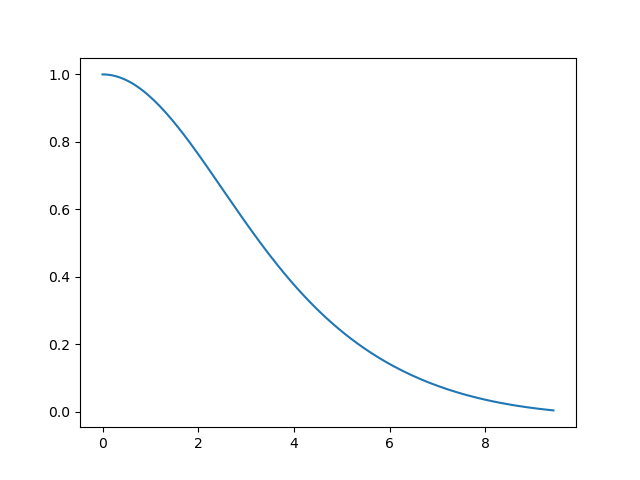
\includegraphics[width=0.72\textwidth]{plot_SW_J1J2_magform_1D.png}
\caption{Kurva magnetic form factor pada gambar yang diberikan. Angka pada sumbu adalah bagian dari gambar sumber, bukan parameter yang dimasukkan ke derivasi ini.}
\label{fig:j1j2-form}
\end{figure}

Gambar~\ref{fig:j1j2-form} langsung mengikuti Persamaan~\eqref{eq:form-factor-definition}. Pada momentum kecil, fase $\ee^{\ii\vQ\cdot\bm r}$ hampir seragam pada seluruh awan elektron sehingga kontribusi menjumlah konstruktif dan $f\simeq1$. Ketika momentum membesar, osilasi fase menyebabkan cancellation sehingga kurva turun. Melalui faktor $|f|^2$ pada Persamaan~\eqref{eq:final-intensity}, penurunan ini meredupkan cabang pada momentum besar tanpa mengubah posisi energinya.

\subsection{Mengapa muncul banyak kurva positif dan negatif}

\begin{figure}[H]
\centering
\begin{subfigure}[t]{0.49\textwidth}
\centering
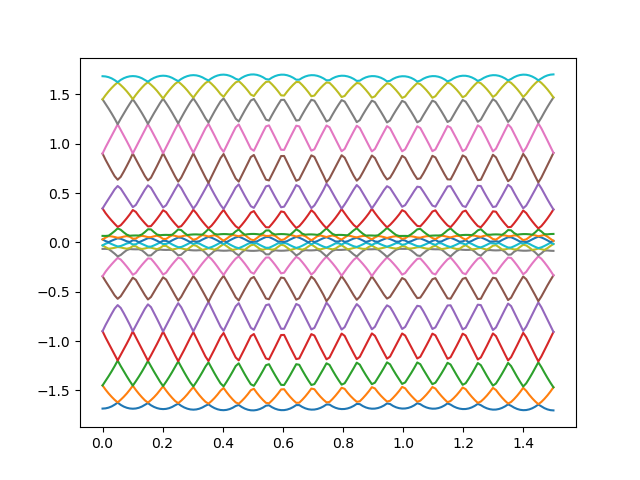
\includegraphics[width=\linewidth]{plot_SW_J1J2_qvsw_1D.png}
\caption{Seluruh eigenvalue matriks dinamik bosonik.}
\end{subfigure}
\hfill
\begin{subfigure}[t]{0.49\textwidth}
\centering
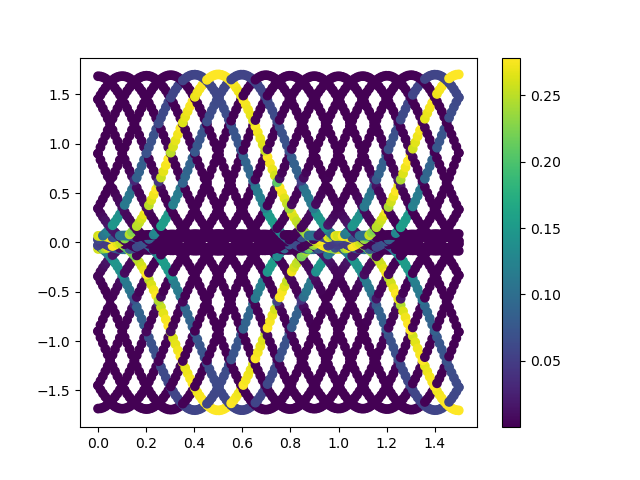
\includegraphics[width=\linewidth]{plot_SW_J1J2_1D.png}
\caption{Eigenvalue yang sama dengan warna sebagai bobot mode.}
\end{subfigure}
\caption{Dispersi model $J_1$--$J_2$ pada gambar yang diberikan.}
\label{fig:j1j2-dispersion}
\end{figure}

Posisi dasar satu cabang spiral diberikan oleh Persamaan~\eqref{eq:spiral-dispersion-Jk} dengan $\mathcal J(k)$ pada Persamaan~\eqref{eq:j1j2-Jk}. Jika spiral direpresentasikan dengan magnetic unit cell berisi $M$ sublattice, momentum fisik dilipat ke reduced Brillouin zone. Secara skematik, cabang terlipat berasal dari
\begin{equation}
\varepsilon_m(q)=\varepsilon(q+G_m),
\end{equation}
dengan $G_m$ reciprocal vector yang berbeda dari magnetic lattice. Karena ada $M$ sublattice, terdapat $M$ cabang energi positif di reduced zone.

Nambu spinor menggandakan dimensi dari $M$ menjadi $2M$ menurut Persamaan~\eqref{eq:nambu-spinor}. Oleh sebab itu plot seluruh eigenvalue menampilkan $M$ cabang positif dan $M$ partner negatif. Simetri atas--bawah pada panel kiri berasal dari pasangan $\pm\varepsilon_n$ pada Persamaan~\eqref{eq:bosonic-eigenproblem}, bukan dari dua jenis eksitasi fisik berbeda.

Panel berwarna memakai informasi eigenvector. Cabang menjadi terang bila $W_n(\vQ)$ pada Persamaan~\eqref{eq:neutron-mode-weight} besar. Cabang terlipat yang gelap tetap solusi eigenvalue, tetapi penjumlahan fase sublattice pada Persamaan~\eqref{eq:mode-amplitude} hampir saling membatalkan. Inilah alasan grafik berwarna menonjolkan hanya beberapa lintasan halus dari sekumpulan besar garis eigenvalue.

\subsection{Peta intensitas dan hubungan pusat puncak dengan dispersi}

\begin{figure}[H]
\centering
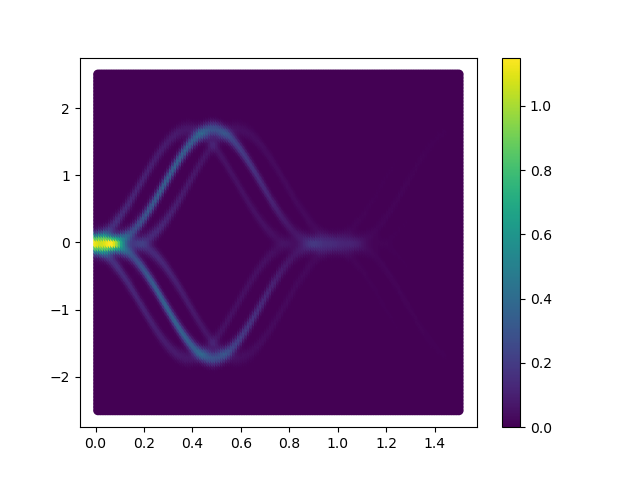
\includegraphics[width=0.76\textwidth]{plot_Intens_SW_J1J2_1D.png}
\caption{Peta intensitas model $J_1$--$J_2$ pada gambar yang diberikan.}
\label{fig:j1j2-intensity}
\end{figure}

Setiap titik terang pada Gambar~\ref{fig:j1j2-intensity} berasal dari satu suku dalam Persamaan~\eqref{eq:final-intensity}. Untuk momentum tetap, Gaussian mode $n$ berpusat di
\begin{equation}
\omega=\omega_n(q)=\frac{\varepsilon_n(q)}{\hbar}.
\end{equation}
Jadi garis tengah pita terang harus berimpit dengan cabang terang pada Gambar~\ref{fig:j1j2-dispersion}. Ketebalan vertikal pita ditentukan oleh $\sigma$ pada Persamaan~\eqref{eq:normalized-gaussian}; $\sigma$ mengubah lebar, bukan lokasi pusat puncak.

Kecerahan sepanjang pita ditentukan oleh produk
\begin{equation}
|f(\vQ)|^2\,W_n(\vQ)\,\mathcal B_n(T).
\end{equation}
Karena form factor menurun terhadap momentum, bagian momentum besar dapat lebih redup meskipun eigenvalue tetap ada. Intensitas kuat dekat energi rendah berasal dari mode Goldstone atau mode hampir-Goldstone yang memenuhi $\varepsilon_n\simeq0$, ditambah bobot matrix element yang tidak nol.

Bagian energi negatif pada gambar dapat dipahami dengan dua cara yang harus dibedakan. Jika yang diplot adalah seluruh spektrum BdG, ia adalah partner Nambu $-\varepsilon_n$. Jika yang diplot adalah structure factor fisik pada temperatur hingga, sisi $\omega<0$ adalah proses energy-gain dan bobotnya harus memenuhi detailed balance. Karena itu interpretasi kuantitatif sisi negatif memerlukan definisi plotting yang eksplisit.

\section{Membaca grafik \texorpdfstring{$J_1$--$D$}{J1--D} langsung dari persamaan}

\subsection{Dispersi, chirality, dan band folding}

\begin{figure}[H]
\centering
\begin{subfigure}[t]{0.49\textwidth}
\centering
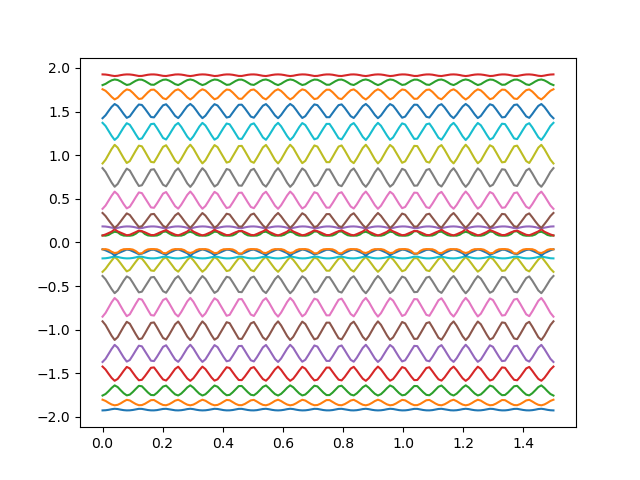
\includegraphics[width=\linewidth]{plot_SW_J1DM_qvsw_1D.png}
\caption{Seluruh pasangan eigenvalue BdG.}
\end{subfigure}
\hfill
\begin{subfigure}[t]{0.49\textwidth}
\centering
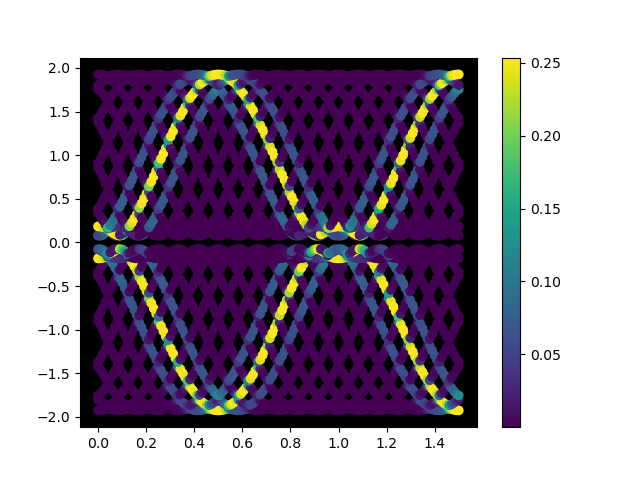
\includegraphics[width=\linewidth]{plot_SW_J1DM_1D.png}
\caption{Eigenvalue dengan bobot mode sebagai warna.}
\end{subfigure}
\caption{Dispersi model exchange--DMI pada gambar yang diberikan.}
\label{fig:j1d-dispersion}
\end{figure}

Pitch tidak dipilih secara arbitrer, tetapi mengikuti Persamaan~\eqref{eq:j1d-pitch}. Setelah pitch diketahui, kombinasi $C_Q=J_1\cos Q+D\sin Q$ menentukan $A_D$ dan $B_D$, lalu posisi cabang mengikuti Persamaan~\eqref{eq:j1d-dispersion}. Tanda $D$ mengubah tanda $Q$, sehingga membalik handedness spiral.

Seperti model sebelumnya, banyaknya garis pada panel kiri berasal dari dua operasi berbeda:
\begin{enumerate}
\item magnetic unit cell multisublattice melipat cabang fisik menjadi $M$ cabang positif;
\item basis Nambu menambahkan $M$ partner negatif.
\end{enumerate}
Warna pada panel kanan tidak berasal dari energi, melainkan dari matrix element Persamaan~\eqref{eq:mode-amplitude}--\eqref{eq:neutron-mode-weight}. Karena rotasi spiral mengandung fase $Q$, operator spin global mencampur momentum lokal $q$ dengan momentum global yang bergeser $q\pm Q$. Akibatnya bobot terang dapat mengikuti envelope yang jauh lebih sederhana daripada kumpulan cabang terlipat.

\subsection{Peta intensitas positif}

\begin{figure}[H]
\centering
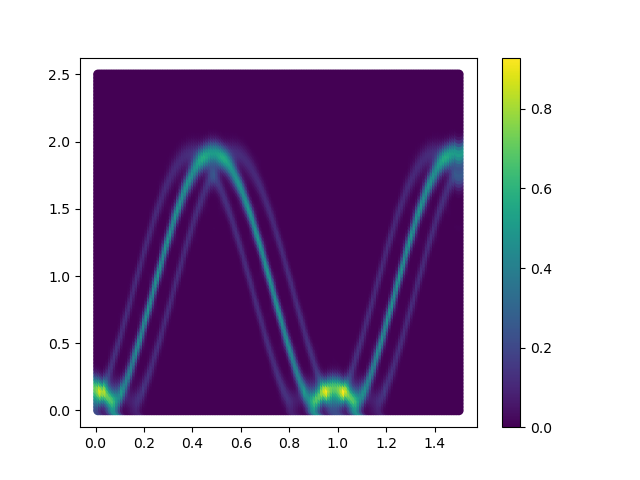
\includegraphics[width=0.76\textwidth]{plot_Intens_SW_J1DM_1D.png}
\caption{Peta intensitas energi positif model exchange--DMI pada gambar yang diberikan.}
\label{fig:j1d-intensity}
\end{figure}

Pita terang pada Gambar~\ref{fig:j1d-intensity} berpusat pada solusi positif Persamaan~\eqref{eq:j1d-dispersion} setelah band folding dan transformasi kembali ke momentum global. Hubungannya dengan panel dispersi adalah
\begin{equation}
\text{garis tengah pita terang}
\Longleftrightarrow
\varepsilon_n(q)>0
\quad\text{dengan}\quad
W_n(\vQ)\ \text{besar}.
\end{equation}
Cabang eigenvalue berwarna gelap tidak hilang dari Hamiltonian; kontribusinya kecil karena projector polarisasi, interferensi sublattice, atau komponen eigenvectornya tidak cocok dengan operator spin yang diukur.

Peta ini hanya memperlihatkan energi positif. Oleh sebab itu partner Nambu negatif yang tampak pada Gambar~\ref{fig:j1d-dispersion} tidak muncul. Broadening mengubah delta function menjadi pita dengan lebar hingga, sedangkan lokasi maksimum tetap mengikuti $\omega_n(q)$.

\section{Urutan komputasi yang mengikuti derivasi}

Untuk mengubah persamaan menjadi kode tanpa melompat langkah, gunakan urutan berikut:
\begin{enumerate}
\item Pilih Hamiltonian dan satu konvensi bond: bond unik tanpa $1/2$, atau jumlah terarah dengan $1/2$.
\item Minimalkan $E_{\mathrm{cl}}$ untuk memperoleh $Q$; gunakan Persamaan~\eqref{eq:j1j2-pitch} atau \eqref{eq:j1d-pitch} untuk dua model di sini.
\item Tentukan $M$ hanya setelah periodisitas spiral ditetapkan. Untuk spiral komensurat $Q=2\pi/p$, ambil $M=p$.
\item Bangun $R_r$ dari Persamaan~\eqref{eq:rotation-matrix} dan coupling lokal $\mM_{rs}$ dari Persamaan~\eqref{eq:local-coupling}.
\item Hitung $T_{rs}$, $P_{rs}$, serta onsite term dari Persamaan~\eqref{eq:bond-order2}--\eqref{eq:P-coefficient}.
\item Jumlahkan seluruh suku linear dan verifikasi $\lambda_r=0$. Jangan melanjutkan jika residual linear belum hilang.
\item Terapkan fase Fourier sesuai displacement bond menggunakan Persamaan~\eqref{eq:fourier-normal-bond} dan \eqref{eq:fourier-pair-bond}.
\item Susun $A(q)$ dan $\Delta(q)$, lalu periksa Hermiticity dan pairing symmetry pada Persamaan~\eqref{eq:bdg-consistency}.
\item Selesaikan $\eta\mH_{\mathrm{BdG}}t_n=\varepsilon_nt_n$, bukan eigenproblem Hermitian biasa, lalu normalkan eigenvector dengan Persamaan~\eqref{eq:paraunitary-normalization}.
\item Ambil cabang positif untuk energi fisik. Jika seluruh $2M$ eigenvalue diplot, labeli cabang negatif sebagai partner Nambu.
\item Bangun amplitudo mode menggunakan Persamaan~\eqref{eq:mode-amplitude}, termasuk fase posisi basis $\bm\tau_r$.
\item Kontraksikan tensor mode dengan projector polarisasi, kalikan $|f|^2$ serta faktor Bose, kemudian broaden dengan Gaussian ternormalisasi untuk memperoleh Persamaan~\eqref{eq:final-intensity}.
\item Periksa konvergensi dengan memperhalus grid $q$ dan $\omega$; parameter grid adalah keputusan numerik yang terpisah dari parameter Hamiltonian.
\end{enumerate}

\section{Kesimpulan}

Seluruh struktur grafik dapat ditelusuri ke persamaan tertentu. Pitch spiral $J_1$--$J_2$ berasal dari minimum energi klasik Persamaan~\eqref{eq:j1j2-pitch}, sedangkan pitch spiral chiral exchange--DMI berasal dari Persamaan~\eqref{eq:j1d-pitch}. Posisi energi ditentukan oleh eigenproblem bosonik Persamaan~\eqref{eq:bosonic-eigenproblem}. Banyak cabang muncul karena band folding oleh $M$ sublattice, dan pasangan negatif muncul karena penggandaan Nambu menjadi dimensi $2M$. Cabang yang benar-benar terang dipilih oleh eigenvector, rotasi lokal, interferensi fase basis, projector polarisasi, dan form factor melalui Persamaan~\eqref{eq:mode-amplitude}--\eqref{eq:final-intensity}. Gaussian hanya memberi lebar pada puncak; pusatnya tetap berada pada dispersi.

Dengan demikian, grafik bukan objek yang terpisah dari derivasi. Setiap garis terang adalah delta function mode yang telah diberi matrix element dan broadening, sedangkan setiap garis gelap adalah mode matematis dengan bobot scattering kecil. Semua parameter fisik tetap simbolik dan harus ditentukan kemudian dari Hamiltonian material atau data eksperimen yang relevan.

\begin{thebibliography}{9}

\bibitem{semiklasik}
\emph{Notes Spinwave Semiklasik}, catatan internal, bagian model Heisenberg, persamaan gerak, anisotropi, feromagnet, dan antiferomagnet.

\bibitem{kuantum}
\emph{Notes Spinwave Kuantum}, catatan internal, bagian operator tangga, satu spin flip, state momentum, dan transformasi Fourier.

\bibitem{hamiltonian}
\emph{Hamiltonian}, catatan internal, derivasi rotasi lokal, transformasi Holstein--Primakoff, transformasi Fourier, exchange, anisotropi, DMI, medan, dan matriks bosonik.

\end{thebibliography}

\end{document}
